\documentclass[Orbiter User Manual.tex]{subfiles}
\begin{document}

\section{Quickstart}
\label{sec:quickstart}
This section demonstrates how to take off and land with one of Orbiter's default spacecraft, the Delta-glider. If you are using Orbiter for the first time, this will help to familiarise yourself with some basic concepts of spacecraft and camera control. You should also read the rest of this manual, in particular \ref{sec:user_interface} on keyboard and joystick interface, \ref{sec:mfd} on instrumentation, \ref{sec:controls} on spacecraft control and \ref{sec:basic_flight} on basic flight manoeuvres.\\
Make sure you have configured Orbiter before launching your first simulation, in particular the video and joystick parameters (see \ref{sec:launchpad}). Once you have started the Quickstart scenario, you can get the following scenario instructions also on-screen by opening the \textit{Help} window with \Alt\keystroke{F1}.\\
\\
\textbf{Starting:}

\begin{itemize}
\item Select the Checklists\textbackslash Quickstart scenario (see \ref{ssec:scenarios_tab} on scenario selection), and press the \textit{Launch Orbiter} button to launch the scenario. Once the mission has been loaded (this can take a few moments) you will see in front of you runway 33 of the SLF (Shuttle Landing Facility) at the Kennedy Space Center, Cape Canaveral, Florida.
\item You are in control of a Delta-glider, a powerful futuristic spacecraft, aligned with the runway centreline and ready for take-off.
\item You can always exit the simulation by pressing \Ctrl\keystroke{Q} or \Alt\keystroke{F4}, or by clicking Exit on the main menu (\keystroke{F4}). Orbiter saves the current simulation status in the (Current status) scenario, so you can continue your flight later by selecting this scenario.
\end{itemize}

\noindent
\textbf{Camera modes:}\\
You are in an external camera mode, looking towards your ship.

\begin{itemize}
\item You can rotate the camera around your ship by pressing and holding down the \Ctrl key and pressing a cursor key (\DArrow\UArrow\RArrow\LArrow) on the cursor keypad of your keyboard. Alternatively you can press the right button on your mouse and drag the mouse to rotate the camera. Or, if you have a joystick with a direction controller ("coolie hat") you can use that as well.
\item To jump into the cockpit of your glider, press \keystroke{F1}. (\keystroke{F1} always toggles between cockpit and external view of the spacecraft you are controlling).
\item In the cockpit, you can look around by rotating the camera with \Alt\DArrow\UArrow\RArrow\LArrow, or with the right mouse button or the joystick coolie hat.
\item To look straight ahead, press the \Home button.
\item To learn more about camera modes have a look at \ref{ssec:menu_camera}.
\end{itemize}

\noindent
\textbf{Cockpit modes:}

\begin{itemize}
\item At the moment, you are in "virtual cockpit" mode - that is, you are inside a three-dimensional representation of the glider cockpit, with the glass pane of the head-up display (HUD) in front of you, and the instruments and controls arranged around you. If you look back, you can even get a glimpse of your passengers in the cabin behind you!
\item You can switch to a different cockpit mode by pressing \keystroke{F8}. Pressing \keystroke{F8} once will open the generic \textit{glass cockpit} mode with only the HUD and two on-screen multifunctional displays. Pressing \keystroke{F8} again will open a 2-D panel mode.
\item The 2-D control panel can be scrolled by pressing a cursor key (\DArrow\UArrow\RArrow\LArrow) on the cursor keypad. To scroll the panel out of the way, press \UArrow. You should now be able to see the runway stretching in front of you. Scrolling the panel is useful if you want to see more of your surroundings. Also, if the panel is larger than your simulation window, you can scroll different parts of the panel into view.
\item If the native resolution of the panel is larger than your simulation window, you can use the mouse wheel to zoom the panel view in and out (this feature may not be supported by all spacecraft types).
\item Some spacecraft have more than a single panel which can be accessed by pressing \Ctrl in combination with a cursor key. If you press \Ctrl\UArrow, you will see the glider's overhead panel with some additional controls. Pressing \Ctrl\DArrow switches back to the main panel.
\item Not all spacecraft types support 2-D panels or 3-D virtual cockpits, but the generic glass cockpit mode is always available.
\item You can find more information on cockpit modes in \ref{sec:cockpit_views}.
\end{itemize}

\noindent
\textbf{MFD instruments:}\\
The most important and versatile instruments are the two \textit{multifunctional displays} (MFDs) in the centre of the instrument panel. Each MFD consists of a square LCD screen and buttons along the left, right and bottom edges.

\begin{itemize}
\item MFDs can be set to different modes: With the mouse, left-click the SEL button at the bottom edge of one of the MFDs. (Alternatively, you can press \Shift\keystroke{F1}. MFD keyboard interfaces always use \Shift key combinations, where the left \Shift key controls the left MFD, and the right \Shift key controls the right MFD). You will see a list of available modes.
\item Click on one of the buttons along the left or right edge to select the corresponding mode. If you click the top-left button, the MFD switches to \textit{Orbit} mode.
\item If you want to select a mode via keyboard, press \Shift\keystroke{F1}+\Shift[letter], where [letter] is the keyboard character listed in grey next to the MFD mode in the selection page.
\item Most modes have additional settings and parameters that can be controlled with the buttons as well. The button labels change to indicate the various mode functions. For example, the \textit{Orbit} mode has a button labelled TGT. This can be used to display the orbit of a target object. Click this button - you will see a dialog box to select a target object. Press \Enter, type iss in the text box, and press \Enter again. This will show the orbital parameters of the International Space Station in the MFD display.
\item To see a short description of the available mode functions, click the MNU button at the bottom of the MFD (alternatively, use \Shift\keystroke{'}).
\item A description of standard MFD modes can be found in \ref{sec:mfd}. Orbiter can also be extended with add-on MFD modes, so you may see additional modes in the list.
\item For now, switch the left MFD to \textit{Surface} mode, and the right MFD to \textit{HSI} mode.
\end{itemize}

\noindent
\begin{figure}[H]
	\centering
	\subfigure{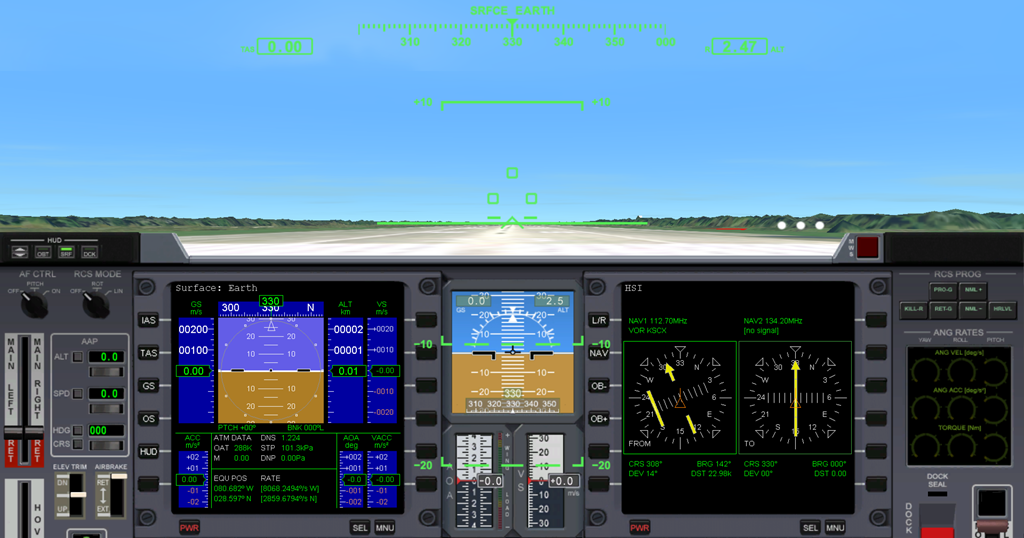
\includegraphics[width=0.99\textwidth]{start_dg_mfd.png}}
\end{figure}

\noindent
\textbf{Take-off:}\\
Your glider is capable of runway take-offs and landings on Earth (and on any other planet, if the atmospheric density is sufficient to provide aerodynamic lift).

\begin{itemize}
\item For take-off, engage main engines at full thrust. You can do this by pushing the \textit{Main} engine sliders at the left of the panel to the top using the mouse. Make sure you push both sliders simultaneously by clicking between them. If you engage only one of your engines, you will quickly veer off the runway into the ditch! (Although you \textit{can} take-off with just one main engine, using thrust vectoring and a lot of rudder - a challenge for another day.)
\item Your spacecraft will start to roll. You can check the speed (in m/s) on the airspeed indicator of the Surface MFD (the tape left of the artificial horizon), or on the HUD - the value in the green box at the top left of the screen.
\item When the airspeed reaches 150 m/s, pull back on the joystick to rotate, or press and hold \keystroke{2}$_{Num}$.
\item Once clear of the runway, press \keystroke{G} to raise the landing gear.
\end{itemize}

\noindent
\begin{figure}[H]
	\centering
	\subfigure{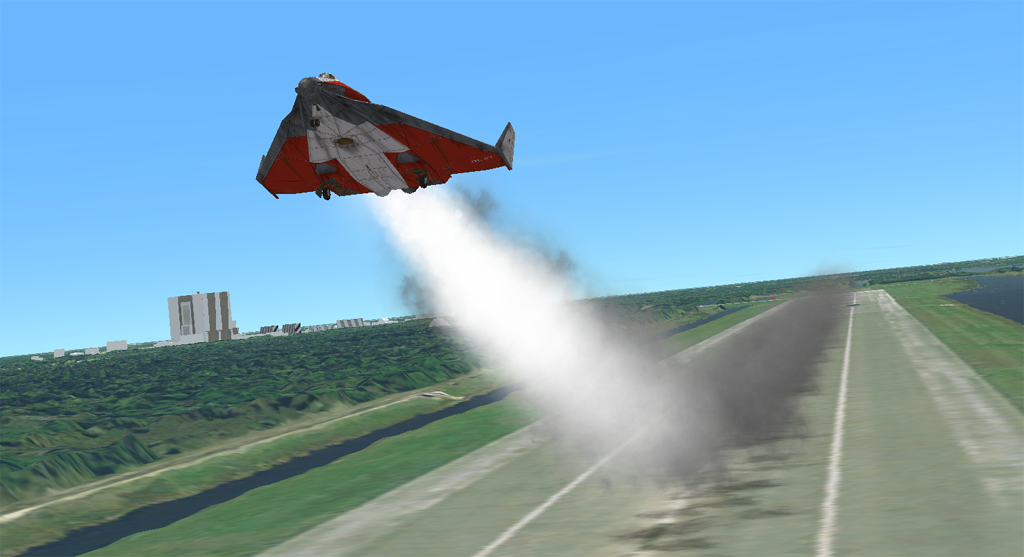
\includegraphics[width=0.99\textwidth]{start_dg_takeoff.png}}
\end{figure}

\noindent
\textbf{Atmospheric flight:}\\
In the lower atmosphere, the glider behaves very much like an aircraft. Try the joystick controls for pitch, yaw and roll to get a feeling for the handling at different altitudes. Without a joystick, you can use the numerical keypad (\keystroke{2}/\keystroke{8}$_{Num}$ for pitch, \keystroke{1}/\keystroke{3}$_{Num}$ for yaw, and \keystroke{4}/\keystroke{6}$_{Num}$ for roll). The glider has powerful rocket engines, but their performance depends on atmospheric pressure (at very low altitudes, it will not even go supersonic).\\
This is a good time to try different camera modes. Open the \textit{Camera} dialog (\Ctrl\keystroke{F1}) and check the effect of different track modes and field of view (FOV) settings.\\
\\
\textbf{Landing:}

\begin{itemize}
\item Go around and approach runway 33 of the SLF from the south. Line up with the runway. Your HSI instrument helps maintain the correct approach path and slope. One of its two displays should already be tuned to the runway ILS system. The HSI contains a course pointer, deviation and glideslope indicator. It works like a standard aircraft instrument, so you may already be familiar with its use. If not, check \ref{ssec:mfd_hsi} for details.
\item As you approach the runway, you will see PAPI and VASI landing aids in front of and beside the runway (see \ref{ssec:basic_landing}). The PAPI is of limited use here, because it is adjusted to the Space Shuttle's steep descent slope of 20°.
\item Throttle back and engage airbrakes (\keystroke{B} to engage by 1/2 step, \Alt\keystroke{B} to retract by 1/2 step) to reduce speed. Lower the landing gear (\keystroke{G}) at speed < 300 m/s.
\item After touchdown, engage left and right wheel brakes (\keystroke{,} and \keystroke{.} simultaneously) once below 150 m/s until you come to a full stop.
\end{itemize}

\noindent
\textbf{Space flight:}\\
So far we have treated the glider much like a conventional aircraft. Now it is time to aim a bit higher ...

\begin{itemize}
\item Take off as before. Turn east (use the compass ribbon at the top edge of the HUD, or the one in the Surface MFD display) and pitch up to 50°.
\item As you gain altitude, you will notice that your craft starts behaving differently, due to the reduction in atmospheric pressure. One of the effects is a loss of lift, which causes the flight path indicator (the $\oplus$ HUD marker) slowly to drift down. Another effect is the loss of response from your aerodynamic control surfaces.
\item At about 40 km altitude your glider will start to drop its nose even while you are pulling back on the stick. That isn't a problem for now - we have already left the denser parts of the atmosphere, and need to pick up horizontal speed to enter orbit anyway, so the levelling of the trajectory is a typical ascent profile for spacecraft - but before the flight path drops too low and you start to lose altitude, it is time to activate the RCS (Reaction Control System) by clicking on the right of the \textit{RCS Mode} dial (on the right side of the instrument panel) or by pressing \Ctrl\keystroke{/}$_{Num}$. You are now controlling your craft with attitude thrusters. The controls for pitch, yaw and roll remain the same, but the handling will feel different - without atmospheric friction, your craft will continue rotating until an opposite force is applied. If you lose control, the \keystroke{5}$_{Num}$ key is your friend. It will automatically engage RCS thrusters until any rotation is cancelled out (the \textit{killrot} autopilot mode).
\item Side note: You can fly most of your ascent trajectory with the Delta-glider without activating RCS along the way. In fact, at this point you could probably just take your hands off the controls and leave the glider to its own devices, relying on the equilibrium between speed and atmospheric density to take you on a "natural" ascent profile. Try it later! You \textit{will} need RCS later on to set up the final, orbit circularisation burn.
 \item Pitch down to about 20° to shift emphasis from gaining altitude to gaining tangential velocity. Your flight path indicator (which tells you the direction your vessel is actually going) should stay above 0°.
\item Now is a good time to activate the \textit{Orbit} mode in one of your MFDs. This shows the shape of your current orbit (the green ellipse) in relation to the planet surface (they grey circle), together with a list of orbital parameters along the left side of the display. You should switch the display to \textit{current orbital plane} projection mode, by clicking the PRJ button until Prj SHP is shown in the top right corner of the display. Also select altitude readouts by clicking the DST button so that the PeR and ApR entries in the data column change to PeA and ApA (periapsis altitude and apoapsis altitude above ground), respectively.
\item At the moment, your orbit will be a rather eccentric ellipse, which for the most part is \textit{below} the Earth's surface. This means that you are still on a suborbital trajectory rather than in a stable orbit. As you keep gaining tangential velocity, the orbit curve will start to expand. Once the green curve is completely above the planet surface (and sufficiently high above the atmosphere) you will have entered orbit. 
\item You probably won't achieve this with a single continuous engine burn. Turn off the engines as soon as the highest point of your orbit (ApA, apoapsis altitude readout) is around 200 km (ApA 200k), even if the projected path is still suborbital. Apart from ApA the most important pieces of information from the Orbit display are periapsis altitude (PeA), eccentricity (Ecc) and orbital velocity (Vel). For this mission, the aim is to enter a stable circular orbit at about 200 km altitude. This requires both ApA and PeA to be at 200k, Ecc close to 0, and a velocity of approximately 7800 m/s.
\item You are now nearly in orbit. All that remains to do is raise the periapsis (the lowest point of the orbit). This is done best when you reach apoapsis, which should be in half an orbit (or around 45 minutes) from your current position. Time to switch into an external camera mode and enjoy the view!
\item It is also a good idea to switch the HUD from surface mode to orbit mode now. Do this by clicking the OBT button in the top left corner of the instrument panel, or by clicking the HUD button on the Orbit MFD. The keyboard shortcut for cycling through HUD modes is \keystroke{H}. In Orbit mode, the HUD flight path ladder is aligned with the orbital plane instead of the horizon plane, and there is a ribbon showing your orbital azimuth angle. It also shows indicators for prograde (the direction of your orbital velocity vector) and retrograde (the opposite direction).
\item When you reach apoapsis, turn your craft prograde. You can see how close you are to apoapsis by checking the ApT (time to apoapsis) value in the Orbit MFD. If it takes too long, press \keystroke{T} to engage time acceleration, and \keystroke{R} to switch back. To turn prograde, you can operate the RCS manually until the prograde HUD marker ($\oplus$) is centred in view, but it is easier to leave it to the automatic attitude control, by simply pressing the Prograde (PRO-G) button in the top right of the instrument panel. The keyboard shortcut is \keystroke{[}.
\item Now fire your main engines again for final orbit insertion. The two parameters to watch are orbit eccentricity (Ecc) and periapsis altitude (PeA). The eccentricity value should get smaller, indicating that the orbit becomes more circular, while the periapsis altitude approaches the apoapsis altitude. Once the eccentricity value reaches a minimum, turn the main engines off. You can also deactivate the prograde altitude by clicking the PRO-G button again.
\item Congratulations! You made it into orbit!
\end{itemize}

\noindent
\begin{figure}[H]
	\centering
	\subfigure{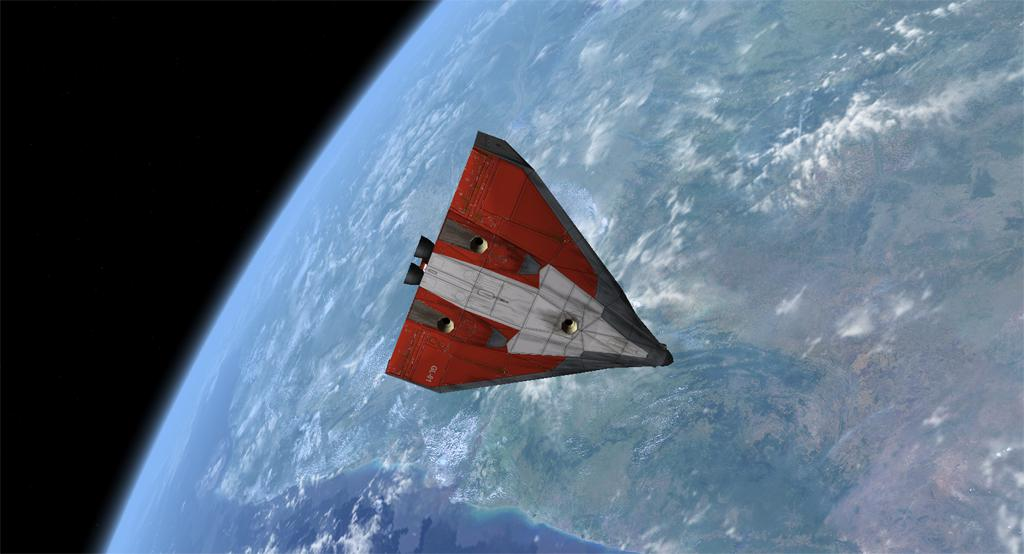
\includegraphics[width=0.99\textwidth]{start_dg_orbit.jpg}}
\end{figure}

\noindent
\textbf{De-orbiting:}\\
Should you ever want to come back to Earth, you need to \textit{de-orbit}. This means to drop the periapsis point to an altitude where the orbit intersects the dense part of the atmosphere, so that your vessel is slowed down by atmospheric friction.

\begin{itemize}
\item De-orbit burns are performed retrograde. Click the \textit{Retrograde} button (RET-G), wait until the vessel attitude has stabilised, and engage main engines.
\item Keep burning until the periapsis point is well below the Earth's surface (PeA < 0), then cut the engines. Strictly speaking, the de-orbit burn must be timed precisely, because too shallow a reentry angle will cause you to skid off the atmosphere, while too steep an angle will turn you into a shooting star. For now we are not concerned with the finer details...
\item Turn prograde again and wait for your altitude to drop. As you enter the lower atmosphere, friction will cause your velocity to decrease rapidly. Reentries are usually performed with a high angle of attack (AOA) to increase friction - about 40° for the Space Shuttle.
\item Once your aerodynamic control surfaces become responsive again you can turn off the RCS system. Your glider has now turned back into an aircraft. (Make sure the airfoil controls are activated if you switched them off in orbit - the AF Ctrl dial must be ON.)
\item You have probably ended up a long way from your launch point at the KSC. Re-entering towards a specified landing point requires some practice in timing the de-orbit burn and the reentry flight path. We'll leave that for a later mission. For now, simply look for a dry patch to land your glider.
\item This completes your first orbital excursion!
You are now ready to try more advanced missions. Try the \textit{DG to ISS} flight described in \ref{ssec:checklist_1} for an orbital rendezvous and docking task. First you might want to learn a bit more about orbital manoeuvres and docking procedures in \ref{sec:basic_flight}.
\end{itemize}


\end{document}
